\documentclass{article}

\usepackage[english]{babel}
\usepackage[letterpaper,top=2cm,bottom=2cm,left=3cm,right=3cm,marginparwidth=1.75cm]{geometry}
\usepackage{amsmath}
\usepackage{graphicx}
\usepackage{float}
\usepackage{subcaption}
\usepackage[colorlinks=true, allcolors=blue]{hyperref}


\usepackage[
backend=biber,
style=alphabetic,
sorting=ynt
]{biblatex}
\addbibresource{SPCSimLib.bib}

\title{Determining the accuracy of FreeRunning mode versus Parallel mode as well as the accuracy of Equi-Width Histograms versus Equi-Depth Histograms under variable Attenuation using SPCSimLib \cite{spc}}
\author{NotSureHowManyPeopleIShouldPutHere \& Elliott H. VanOrman}

\begin{document}
\maketitle

\begin{abstract}
This paper compares the error in results of a Single Photon Camera (SPC) in parallel mode versus freerunning mode, as well as comparing error when using Equi-Width Histograms (EWH) and Equi-Depth Histograms (EDH).
Data was collected using the python library SPCSimLib, specifically by simulating a single SPC pixel, and measuring the error each method produced.
Our analysis showed that when FreeRunning mode was used, the resulting measurements matched with reality more than when parallel mode was used, to a statistically significant level.
from this, we concluded that FreeRunning mode produced more accurate results than parallel mode,
\end{abstract}

\section*{Introduction}

Single Photon Cameras, or 'SPC's for short, are cameras that function similarly to LIDAR, in that they produce 3D photographs by measuring the time it takes for light to travel to a point and bounce back. unlike LIDAR however, SPCs use individual photons instead of lasers.

when a picture is taken, the SPC begins sending out pulses of photons towards the thing it is taking a picture of. when these photons are reflected back onto the detector, it records the timestamp. There are almost always ambient photon levels, however, meaning that while timestamps do cluster around the 'true' time it took photons to reflect back, there are a certain number of 'noise' timestamps due to background illumination. there are multiple methods to determine when the true center of the pulse, called the 'peak' is located. after the 'peak' is located, it is used to determine the distance from the camera of the pixel using the formula \[\frac{T*\frac{1}{2}}{C}\] where $T$ is the time it took for photons to reflect back to the detector and $C$ is the speed of light.

the exact steps of sorting out noise from true varies based on method: When using Equi-Width histograms, a histogram is constructed with buckets of equal width but variable depth. The center of the bucket with the most detections is recorded as the 'peak' of the pulse. When using Equi-Depth histograms, a histogram is constructed with buckets of variable width but equal depth. The center of the bucket with the thinnest width is recorded as the 'peak' of the pulse.

Due to the physical limitations of SPC cameras, however, photon readings over time do not always match reality. when a detector is hit by a photon, it takes a certain amount of time for said detector to log a timestamp. While this time is in progress, the detector cannot record new hits. in other words, a detector cannot start recording a new timestamp until it has finished recording the first, meaning photons that hit the detector during that recording time go undetected. this time is refered to as 'deadtime'

how SPC cameras deal with deadtime also varies based method, or, in this case, Mode. in Parallel mode, detectors are reset at the begining of each cycle, regardless of whether or not they've detected anything. this method leads to photon readings to be skewed to the right. This is due to early photons triggering deadtime, preventing pixels from detecting photons until late into a detection-cycle.  In asynchronous mode, also called freeRun mode, detectors do not reset at the beginning of each cycle, leading to relatively less skewed data.

Additionally, the length the laser will fire (refered to as FWHM, or Full Width at Half Maximum, refering to the length of the curve of intensity of the laser when it fires), also varies, and said length could also affect the error of the laser, as the increaed length of the laser would also increase the width of the 'peak' of the pulse

Unfortunately, due to the skew and issues in data, it often becomes necesary to filter out a certain percent of incoming photons. this filtering is called 'attenuation', and  while it may reduce the overal number of photons hitting an SPC, the fact that any one datapoint blocks other datapoints from being recorded for a period of time causes it to actually increase the amount of photons not blocked by early recordings, reducing the skew  of the data and increasing accuracy.

As I have explained, there are many methods that can be used to receive and interpret data from SPCs, but it has not yet been determined which produces the most accurate results. It was hypothesized that Equi-depth histograms would produce more accurate results than Equi-Width histograms, that asynchronous (non-freerunning) mode would produce more accurate results than parallel (freerunning) mode, and that 1.5 FWHM would produce the same amount of error as 5.0 FWHMs.


\section*{Method}
In order to determine what produced the most accurate results, we used the Python library SPCSimLib \cite{spc} to simulate a pixel of an SPC. to find error, we simulate taking a picture with an SPC. then, we subtract the 'true distance' (the distance from the camera the surface being photographed was in the simulation) from the 'estimated distance' (the distance from the camera of the same surface that the SPC in the simulation estimated). after taking this difference, we normalize it by dividing it by the scale of the distance. This normalized difference is what we are referring to when we say 'error'. To miminize the error in our measurements caused by fluctuations in our error measurements, we do this ten times and take tha average. after taking error measurements for every whole numbered percentage value of attenuation, we put this data into a 'dataset', label it with the settings the SPC used while simulations were being taken, then saved said dataset to \href{https://github.com/yggaraxyg/SPCErrorLowerer/tree/master/RunData/runDataUsedInInitialProject}{this folder in our project's github repo}. we then changed the settings, and repeated the process in order get the data we analyzed. we then graphed this data in the formats shown below for ease of understanding saving them to \href{https://github.com/yggaraxyg/SPCErrorLowerer/tree/master/Graphs}{this folder in our project's github repo}.

\begin{figure}[H]
\centering
\begin{subfigure}[b]{1\textwidth}
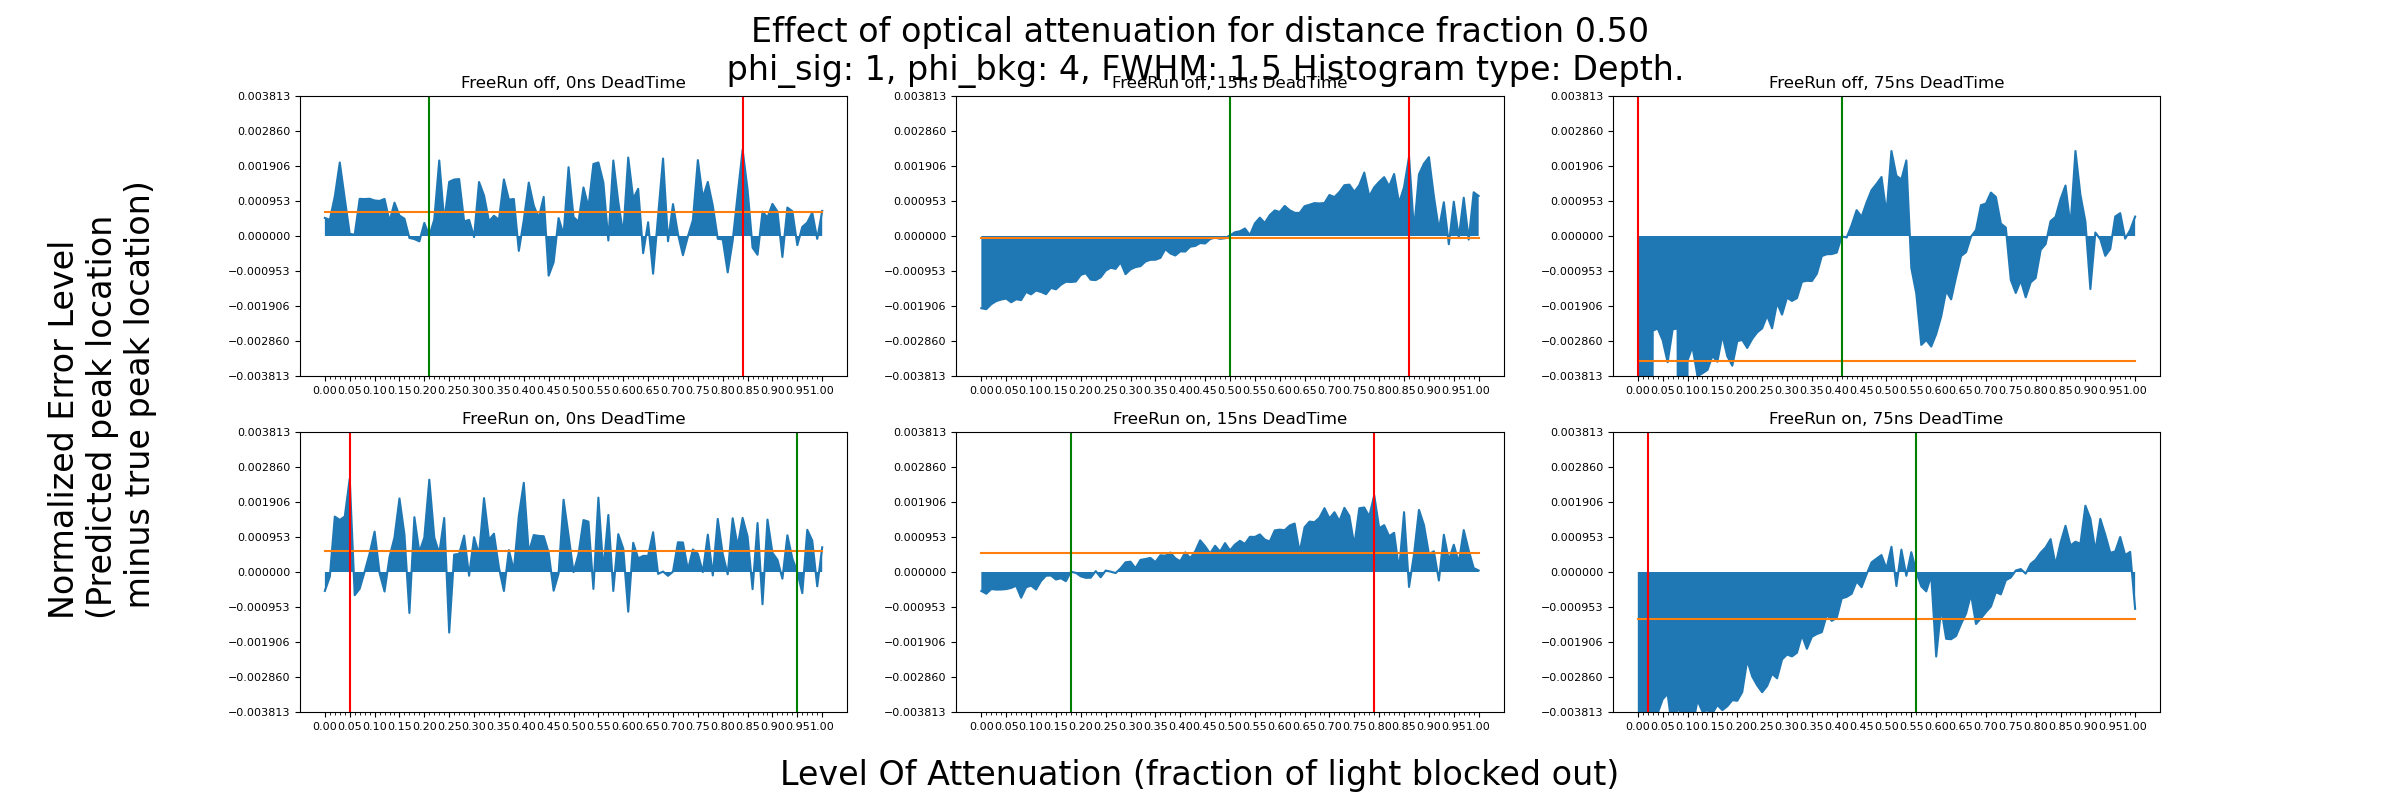
\includegraphics[width=1\linewidth]{SharedyExample.png}
\label{fig:Ng1}
\end{subfigure}
\begin{subfigure}[b]{1\textwidth}
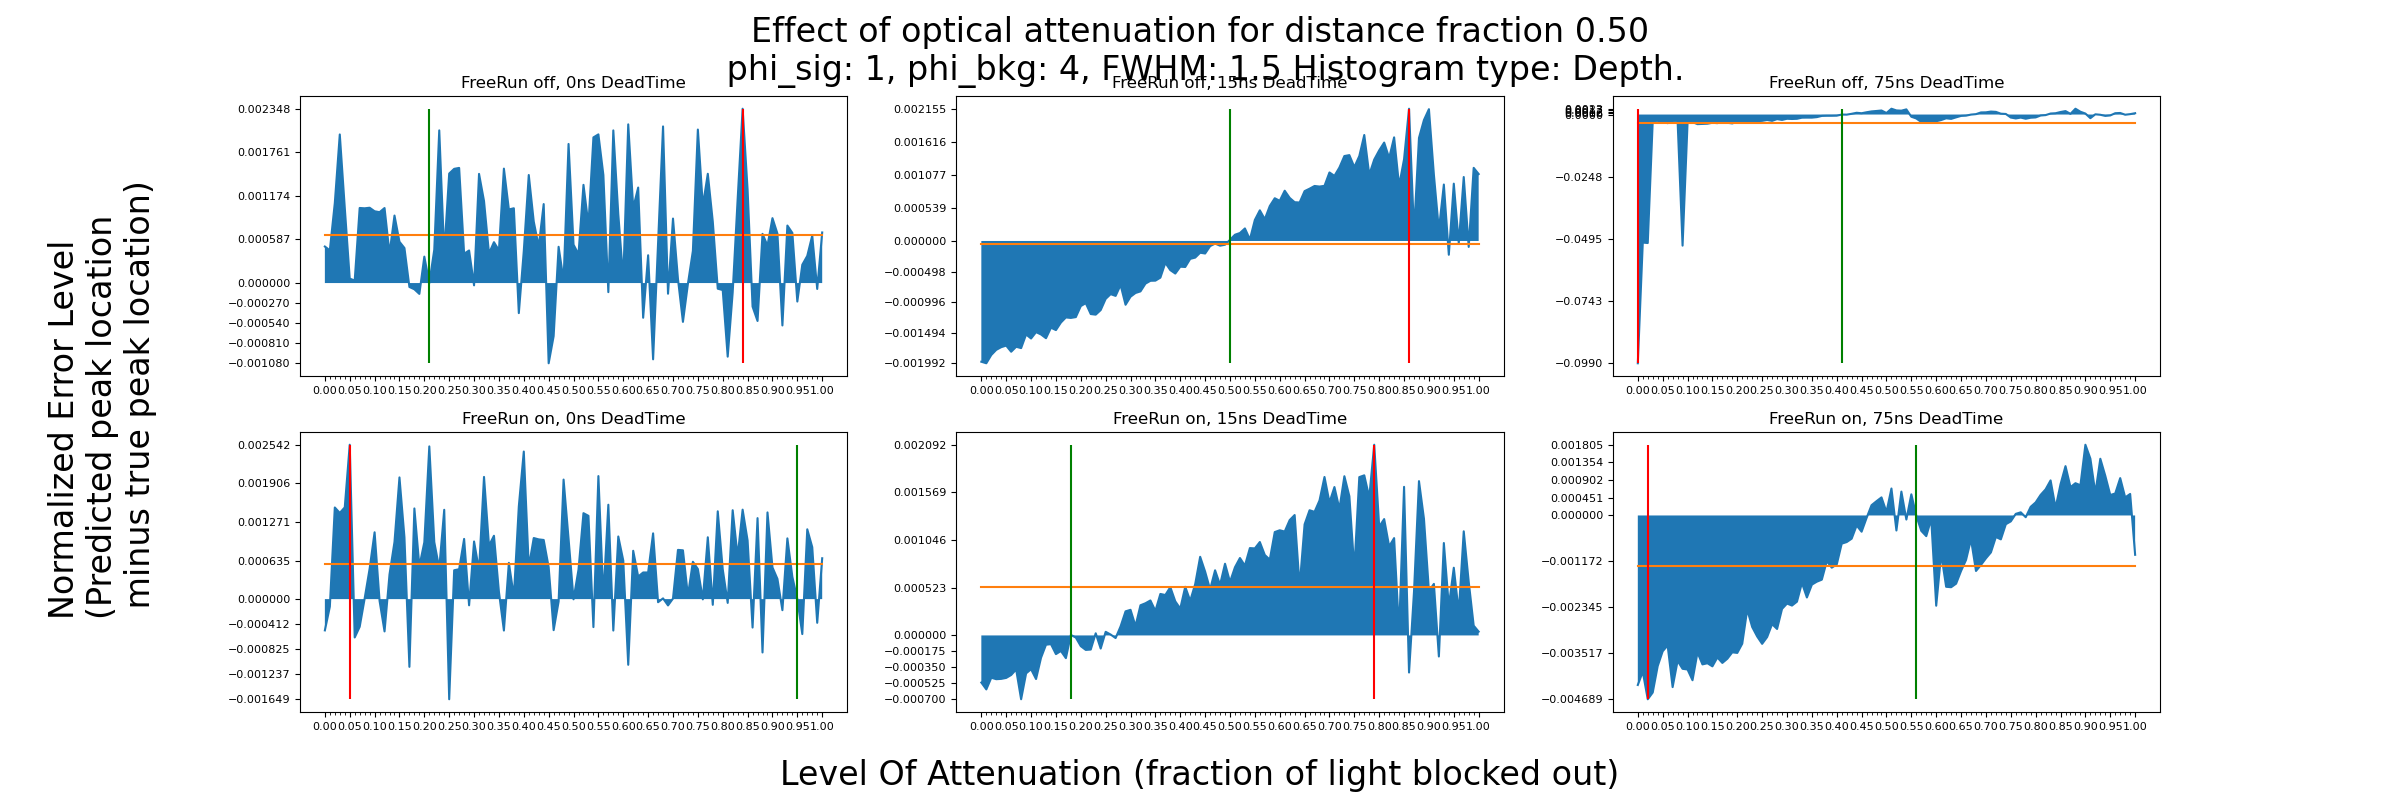
\includegraphics[width=1\linewidth]{ZoomedyExample.png}
\label{fig:Ng2}
\end{subfigure}

\caption{\label{fig:Data}The top graph and the bottom graph present the same data in two different formats. the top graph represents error on the same scale across all graphs, while the bottom represents each dataset with it's own scale. Blue represents normalized error. Orange is the mean error for all attenuation values. Red is the attenuation value which produced the least accurate result. Green is the attenuation value which produced the most accurate result.}

\end{figure}

in addition, we ran statistical analysis on the data to check our hypotheses. to do this, we put all our data in two large datasets for every hyposis, one for each differing state in the hypothesis each state is relevant to. For every hypothesis, we marked the first dataset $d_{1}$ and the second dataset $d_{2}$. we then performed a paired t-test on the data, where each observation's partner was an observation taken under circumstances identical to the first's except for the variable being tested. 

\section*{Results}
Using Paired t-tests, we found the following $T$'s and P-Values for the following alternate hypotheses:
\begin{itemize}
  \item $\mu_{EDH}$\&$\mu_{EWH}$: $T=14.59122$
  \begin{itemize}
    \item $\mu_{EDH}>\mu_{EWH}$: $p=1.79689\times10^{-48}$
    \item $\mu_{EDH}\neq\mu_{EWH}$: $p=3.59378\times10^{-48}$
    \item $\mu_{EDH}<\mu_{EWH}$: $p=1.0$
  \end{itemize}  
  \item $\mu_{F}$\&$\mu_{nF}$: $T=-31.63417$
  \begin{itemize}
    \item $\mu_{F}>\mu_{nF}$: $p=1.0$
    \item $\mu_{F}\neq\mu_{nF}$: $p=1.63522\times10^{-218}$
    \item $\mu_{F}<\mu_{nF}$: $p=8.17611\times10^{-219}$
  \end{itemize}
  \item $\mu_{1.5}$\&$\mu_{5.0}$: $T=-55.67372$
  \begin{itemize}
    \item $\mu_{1.5}>\mu_{5.0}$: $p=1.0$
    \item $\mu_{1.5}\neq\mu_{5.0}$: $p=0$
    \item $\mu_{1.5}<\mu_{5.0}$: $p=0$
  \end{itemize}
\end{itemize}

All alternatve hypotheses with p-values less than 0.01 accepted. graphs showing examples of the accepted hypotheses are as follows:

\begin{figure}[H]
\centering
\begin{subfigure}[b]{1\textwidth}
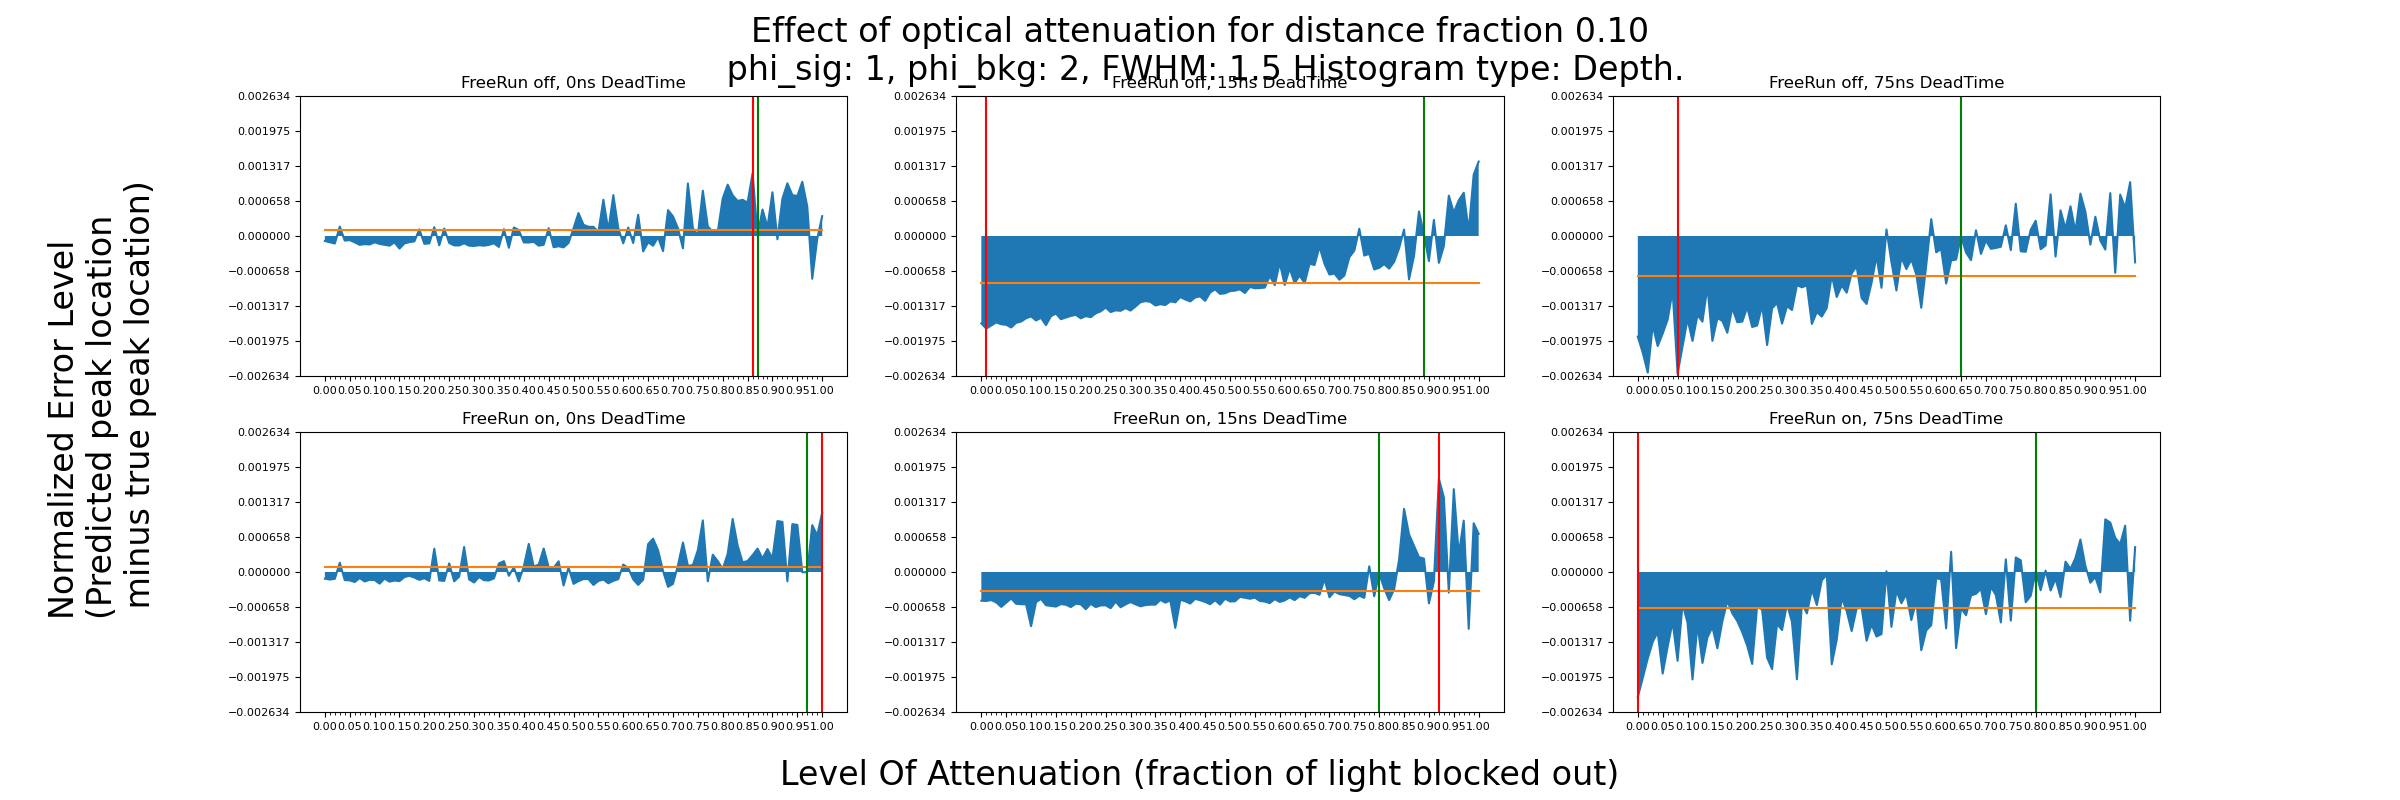
\includegraphics[width=1\linewidth]{depthExample.png}
\label{fig:Depth Example}
\end{subfigure}
\begin{subfigure}[b]{1\textwidth}
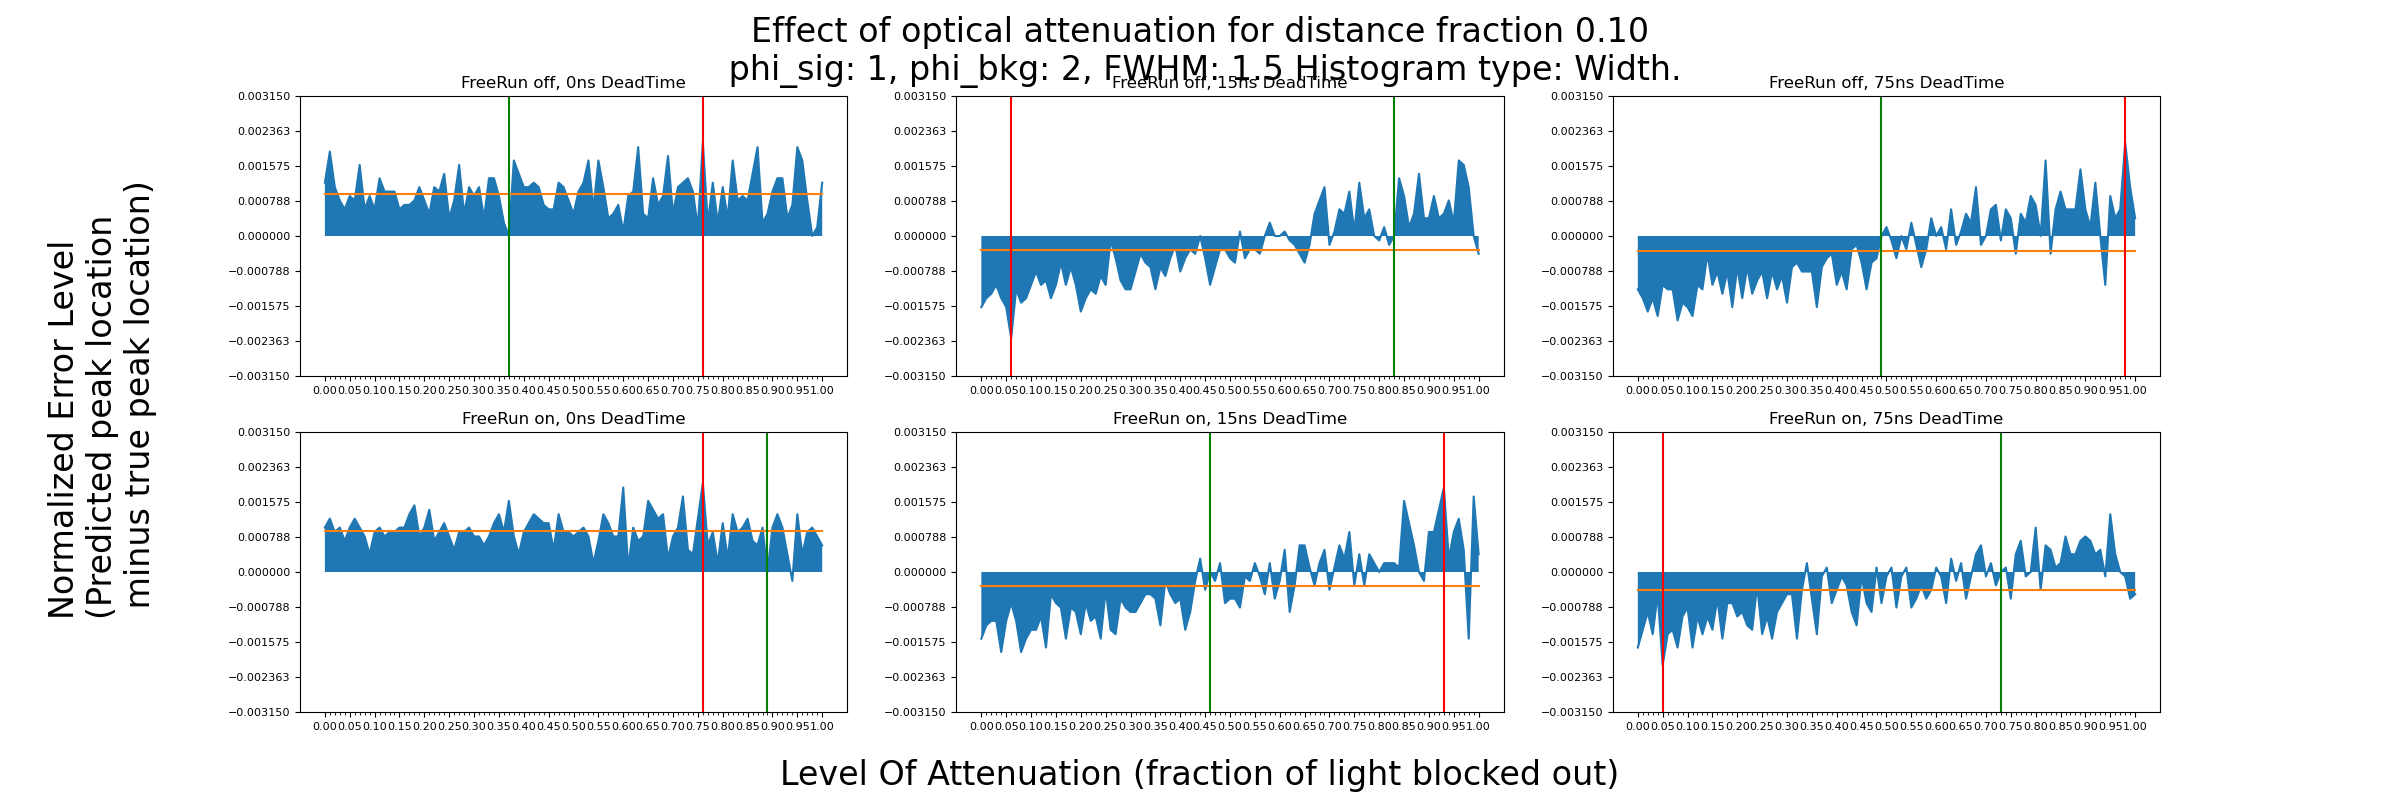
\includegraphics[width=1\linewidth]{widthExample.png}
\label{fig:Width Example}
\end{subfigure}
\caption{\label{fig:histogramComparison}EDH vs EWH}
\end{figure}

\begin{figure}[H]
\centering
\begin{subfigure}[b]{1\textwidth}
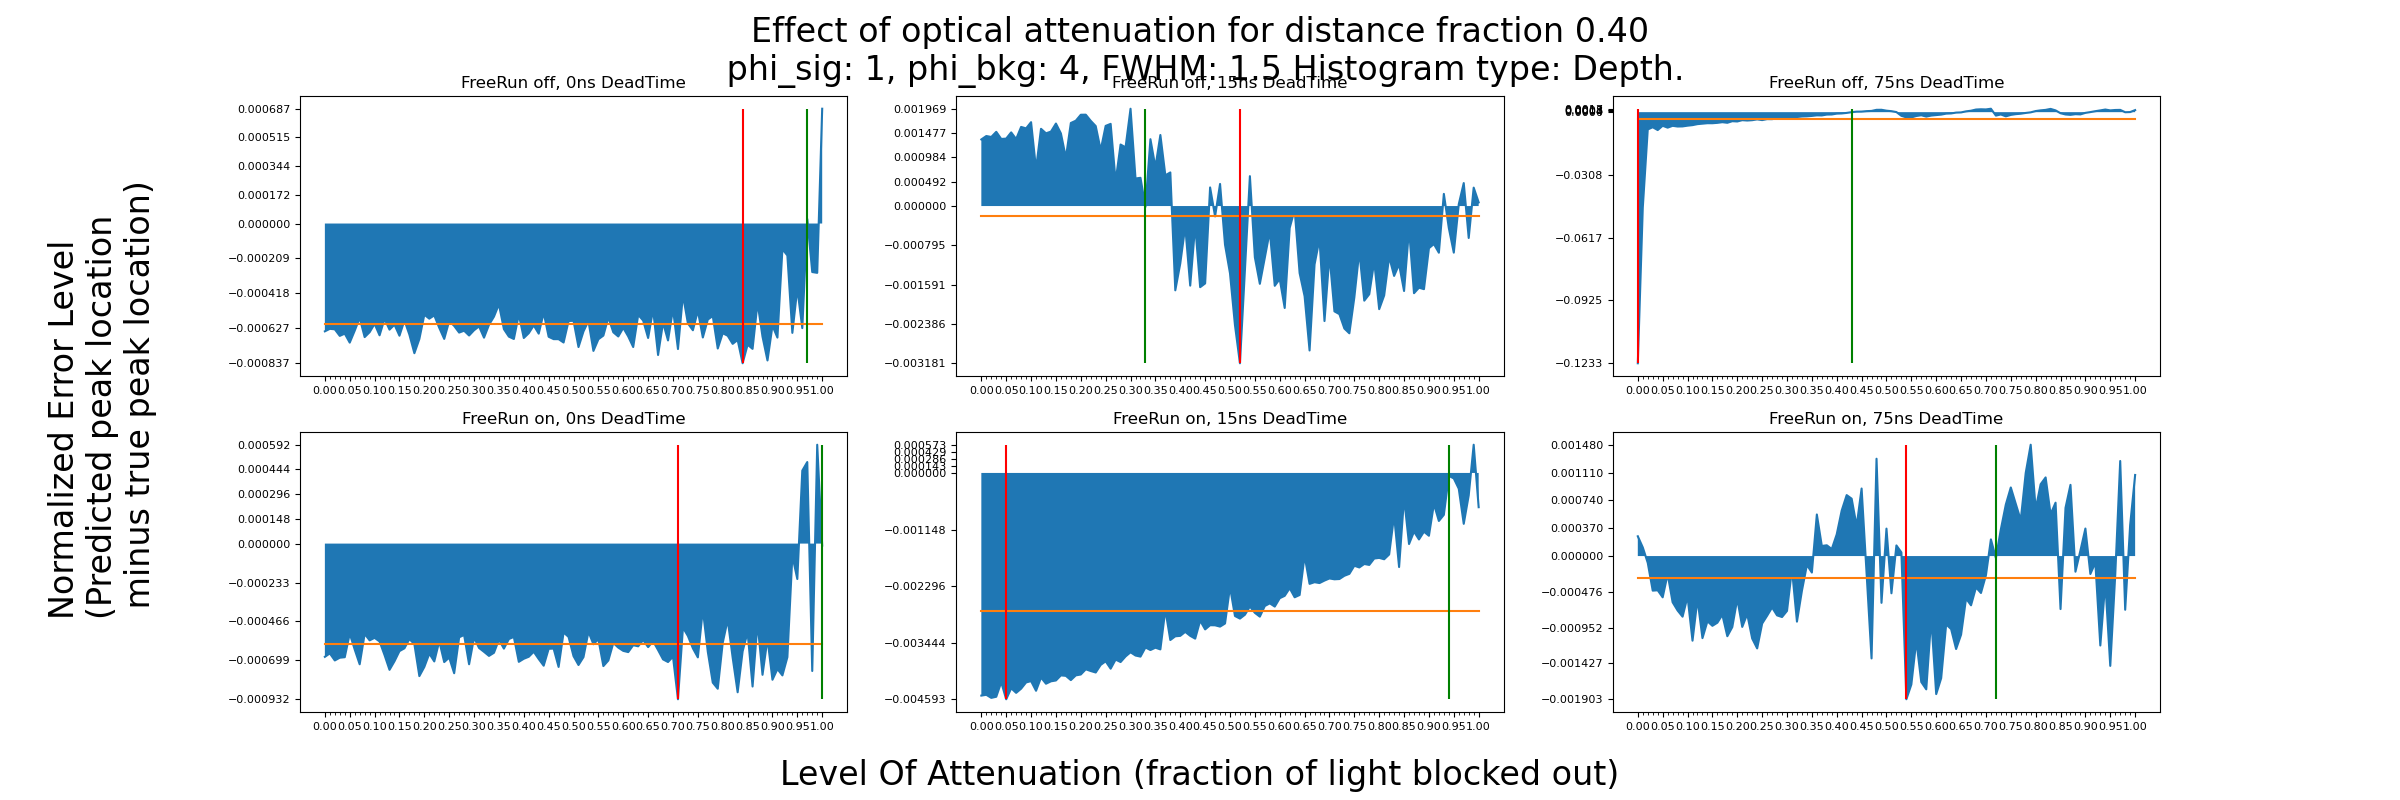
\includegraphics[width=1\linewidth]{zoomedFreeExample.png}
\label{fig:zoomedExample}
\end{subfigure}
\begin{subfigure}[b]{1\textwidth}
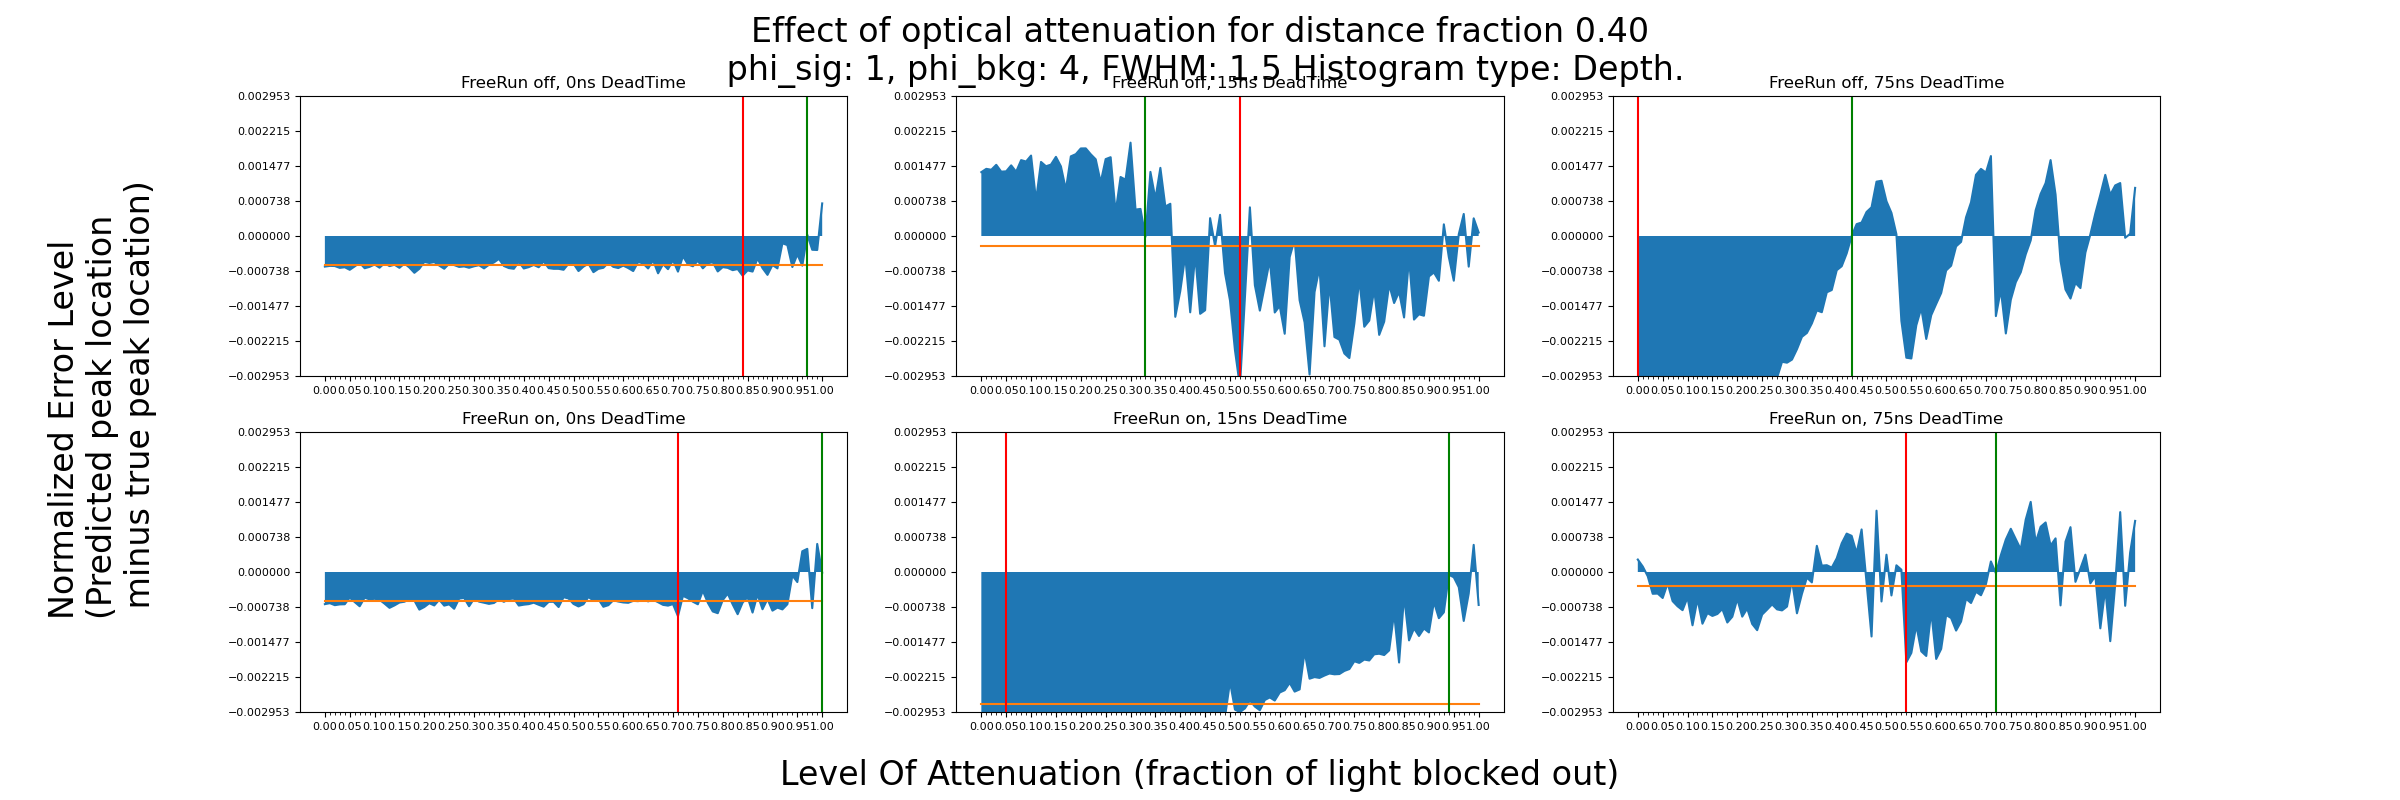
\includegraphics[width=1\linewidth]{sharedFreeExample.png}
\label{fig:sharedExample}
\end{subfigure}
\caption{\label{fig:freerunComparsion}Freerun and non-Freerun on different y axes.}
\end{figure}

\begin{figure}[H]
\centering
\begin{subfigure}[b]{1\textwidth}
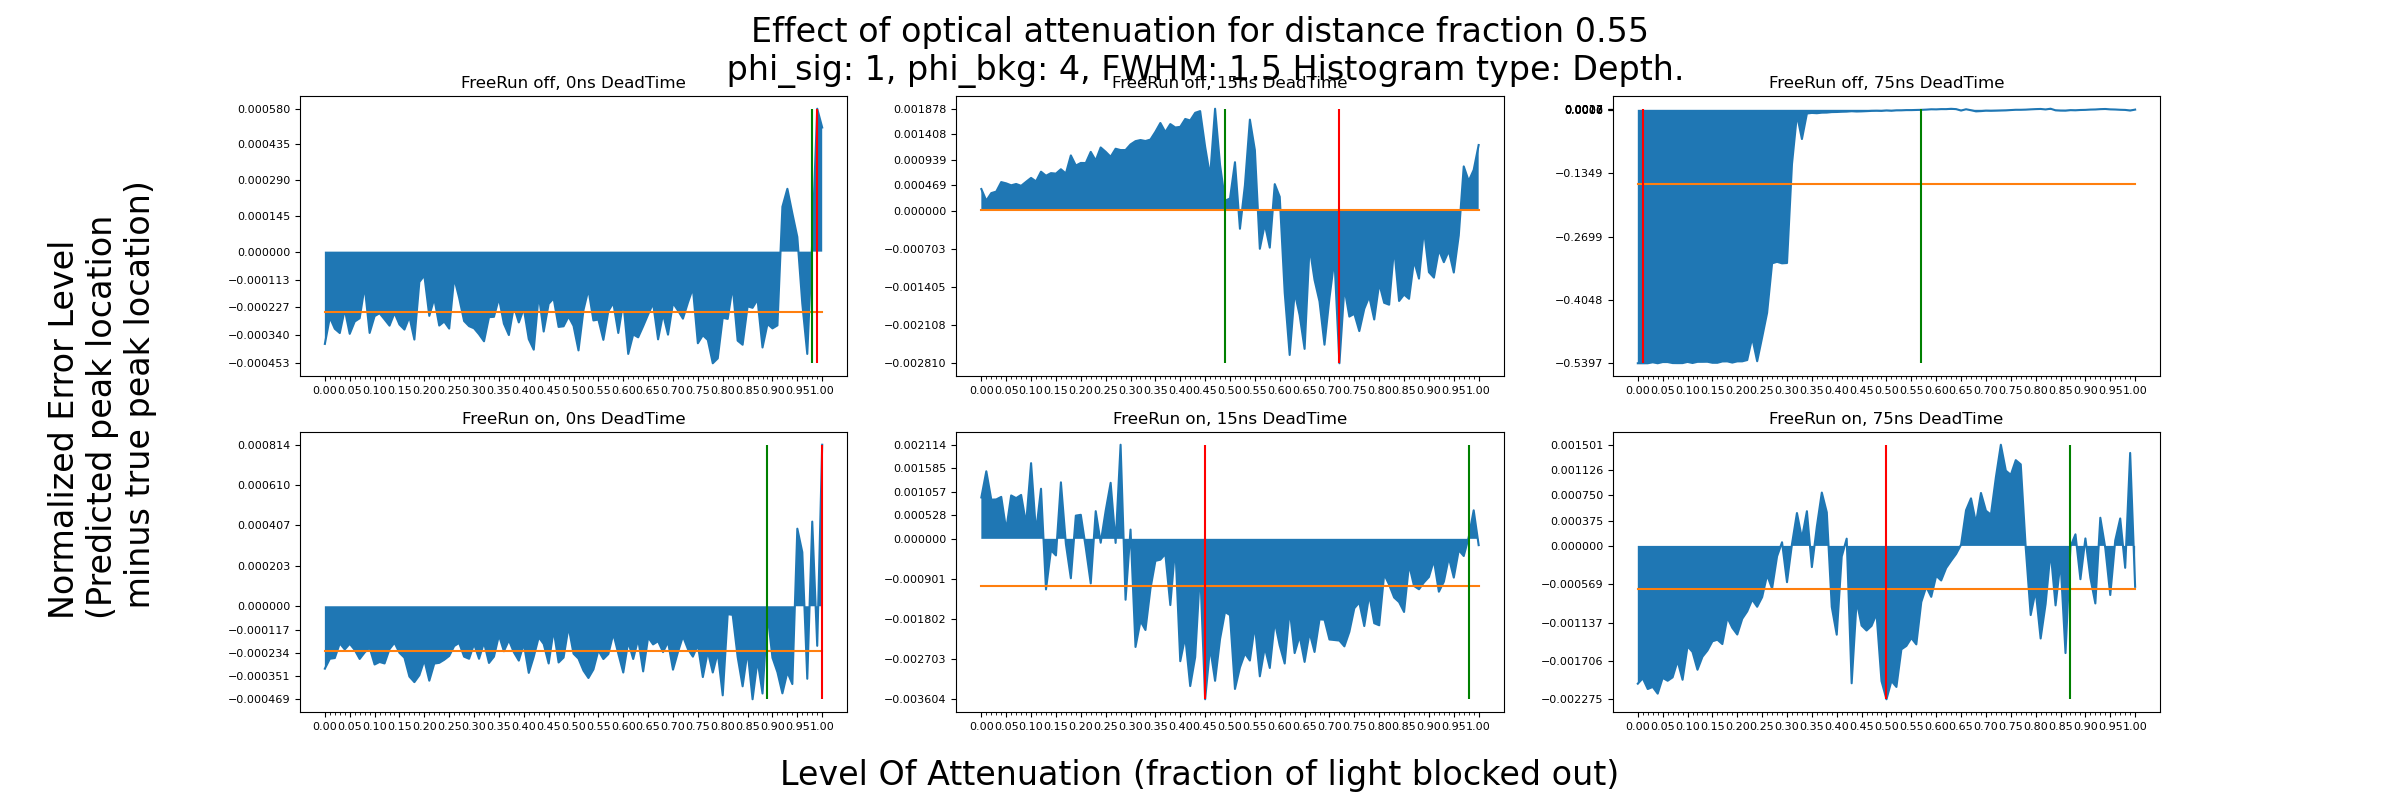
\includegraphics[width=1\linewidth]{1.5Example.png}
\label{fig:1.5Example}
\end{subfigure}
\begin{subfigure}[b]{1\textwidth}
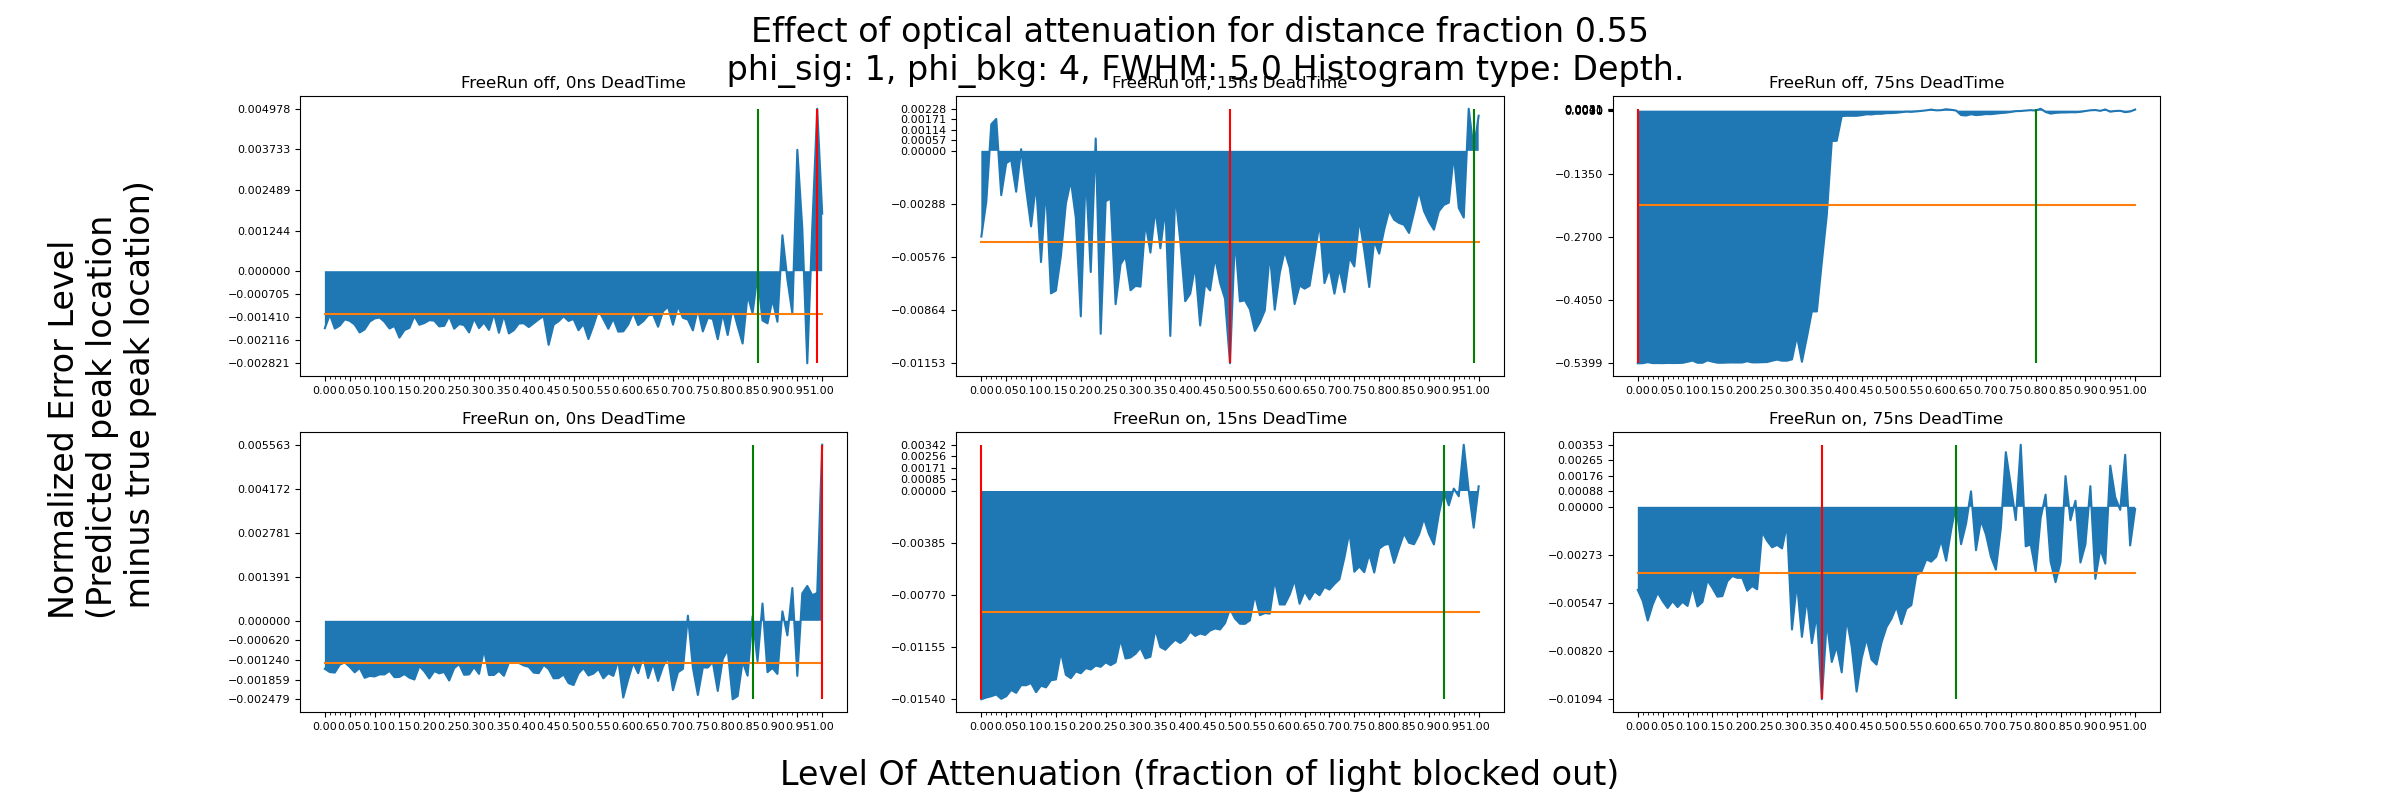
\includegraphics[width=1\linewidth]{5.0Example.png}
\label{fig:5.0Example}
\end{subfigure}
\caption{\label{fig:pulseComparison}1.5 FWHM vs 5.0 FWHM.}
\end{figure}

\section*{Discussion}
In Short, the results show that:
\begin{itemize}
  \item EDH Error Calculation produces more error than EWH Error Calculation, which does not support our hypothesis that EDH Error Calculation produces less error than EWH Error Calculation.
  \item FreeRun simulations produce less error than Non-Freerun simulations, which does support our hypothesis that FreeRun (asynchronous) simulations produce less error than Non-Freerun (parallel) simulations.
  \item 1.5 FWHM simulations produce less error than 5.0 FWHM simulations, which does not support our hypothesis that FreeRun simulations produce less error than Non-Freerun simulations.
\end{itemize}
While some of these results were different from our expectations, they are still explainable observations. some possible (but not necesarily correct) explanations are as follows
\begin{itemize}
\item EDH error calculation, may be prone to overvaluing shorter but wider peaks like the ones produced by skewed data and undervaluing tall but thin peaks like the ones produced at the actual peak, while EWH error calculation simply measures the highest bucket.
  \item FreeRun simulations are less prone to producing skewed data, as the point where individual detectors start detecting photons within a cycle varies, thus allowing photons from later into each cycle hit the detector more often.
  \item shorter FWHM simulations may produce taller, thinner peaks as the photons are clustered closer together, thus makign the peak stand out from the rest of the data more.
\end{itemize}
Our findings have a few implications for practial use of SPCs. the specific implications is that when trying to minimize error while taking SPC photographs...
\begin{itemize}
  \item One should use EWH error caclulation instead of EDH error calculation.
  \item One should use Asynchronous data collection (Freerunningmode) instead of Parallel data collection.
  \item One should set their laser's FWHM to 1.5 instead of 5.0.
\end{itemize}

\section*{Limitations}
All data was collected using the SPCSimLib library, so any flaws in the methods by which it collects data would cause flaws in the data we have analyzed and graphed. additionally, each simulation was prone to it's own fluctuations, and while we did take an average of 10 repeitions to reduce the error in our error measurements (meaning the difference between our average erorr measurements and base reality) there were still fluctuations in the data, despite the relatively clear trends.

\section*{Conclusion}
As Single Pixel Cameras develop and their use increases, it is important to know what settings will allow said SPCs to produce the most accurate pictures. After we repeatedly simulated  individual pixels of SPC cameras across several settings to collect enough data, we found that calculating error with EWH error calculation, Asynchronous Data Collection and 1.5 FWHM lasers produced the most accurate results. This implies that to produce highly-accurate pictures for SPC cameras, one should use said settings. From this, we propose that these become standard settings for SPC cameras,

\printbibliography

\end{document}
